\documentclass[a4paper,
              %boxit,        % check whether paper is inside correct margins
               %titlepage,    % separate title page
            %   refpage       % separate references
            %   biblatex,     % biblatex is used
               keeplastbox,   % flushend option: not to un-indent last line in References
              nospread,     % flushend option: do not fill with whitespace to balance columns
               %hyphens,      % allow \url to hyphenate at "-" (hyphens)
            %   xetex,        % use XeLaTeX to process the file
            %   luatex,       % use LuaLaTeX to process the file
               ]{jacow}
%
% ONLY FOR \footnote in table/tabular
%
\usepackage{pdfpages,multirow,ragged2e} %
\usepackage{physics}
\usepackage{caption}
\usepackage{subcaption}
%
% CHANGE SEQUENCE OF GRAPHICS EXTENSION TO BE EMBEDDED
% ----------------------------------------------------
% test for XeTeX where the sequence is by default eps-> pdf, jpg, png, pdf, ...
%    and the JACoW template provides JACpic2v3.eps and JACpic2v3.jpg which
%    might generates errors, therefore PNG and JPG first
%
\makeatletter%
	\ifboolexpr{bool{xetex}}
	 {\renewcommand{\Gin@extensions}{.pdf,%
	                    .png,.jpg,.bmp,.pict,.tif,.psd,.mac,.sga,.tga,.gif,%
	                    .eps,.ps,%
	                    }}{}
\makeatother

% CHECK FOR XeTeX/LuaTeX BEFORE DEFINING AN INPUT ENCODING
% --------------------------------------------------------
%   utf8  is default for XeTeX/LuaTeX
%   utf8  in LaTeX only realises a small portion of codes
%
\ifboolexpr{bool{xetex} or bool{luatex}} % test for XeTeX/LuaTeX
 {}                                      % input encoding is utf8 by default
 {\usepackage[utf8]{inputenc}}           % switch to utf8

\usepackage[brazil]{babel}

%
% if BibLaTeX is used
%
\ifboolexpr{bool{jacowbiblatex}}%
 {%
  \addbibresource{ipac_references.bib}
  
%   \addbibresource{biblatex-examples.bib}
 }{}
\listfiles
%%
%%   Lengths for the spaces in the title
%%   \setlength\titleblockstartskip{..}  %before title, default 3pt
%%   \setlength\titleblockmiddleskip{..} %between title + author, default 1em
%%   \setlength\titleblockendskip{..}    %afterauthor, default 1em
% \raggedbottom
\begin{document}

\title{Emittance Exchange at Sirius Booster for Storage Ring Injection Improvement}

\author{J. V. Quentino, M. B. Alves\thanks{murilo.alves@lnls.br}, F. H. de Sá \\ Brazilian Synchrotron Light Laboratory (LNLS), 13083-100, Campinas, Brazil}

\maketitle
%
\begin{abstract}
SIRIUS is the new 4\textsuperscript{th} generation storage ring based synchrotron light source built and operated by the Brazilian Synchrotron Light Laboratory (LNLS) at the Brazilian Center for Research in Energy and Materials (CNPEM). Currently, the efficiency of the horizontal off-axis injection system of the storage ring is still not suitable for top-up operation due to a smaller than expected horizontal dynamic aperture. In this work, we report the simulations and experimental results of transverse emittance exchange (TEE) performed at SIRIUS booster by crossing a coupling difference resonance during energy ramp, with the goal of decreasing the injected horizontal beam size and improve the off-axis injection efficiency.
\end{abstract}

\section{Introdução}

The injection system for SIRIUS storage ring (SR) was designed since early stage for beam accumulation with off-axis injection using a single non-linear kicker (NLK)~\cite{Liu:IPAC16-THPMR011}. With this injection scheme, a small horizontal beam size is beneficial to minimize the sampling of non-linear fields at NLK and to allow for high injection efficiency. Thus, SIRIUS booster was designed to achieve a small horizontal emittance of~$\SI{3.5}{\nano\meter\radian}$ at extraction energy of~$\SI{3}{\giga\electronvolt}$~\cite{Liu:IPAC14-WEPRO009}.
 
The SIRIUS NLK was designed to have a peak field at $x_p \approx \SI{-9.0}{\milli \meter}$ and no field at $x=\SI{0}{\milli \meter}$, close to the stored beam. Injection dynamics studies indicated that this field profile would perform the injection with 99\% of efficiency for a beam reaching the NLK at $x_0=\SI{-8.5}{\milli \meter}$~\cite{Liu:IPAC16-THPMR011}.

% Injection dynamics studies made in SIRIUS design showed that, considering a reasonable estimate of horizontal dynamic aperture left limit $x_l=\SI{-9.5}{\milli\meter}$ and the injection position at $x_0=\SI{-8.5}{\milli \meter}$, the injection would be performed with 99\% of efficiency~\cite{Liu:IPAC16-THPMR011, Dester:IPAC17-WEPIK052}.

However, dynamic aperture measurements revealed a horizontal aperture of about $\SI{-8.5}{\milli \meter}$, which is worse than the $\SI{-9.5}{\milli \meter}$ value predicted by the nominal model \cite{Dester:IPAC17-WEPIK052} and is strictly close to the planned injection position,
% , %
% which leaves a small margin between the injection position and the dynamic aperture limit, %
obliging us to move the injection position to $x_0=\SI{-8.0}{\milli \meter}$. As a consequence, even with the booster delivering a beam with small transverse sizes and the booster-to-SR transport line optics being optimized for partially compensate the defocusing effect made by nonlinear fields, the horizontal spread induced by the NLK in the actual injection position is sufficient to reduce the injection efficiency to about $\SI{86}{\%}$, with a large pulse-to-pulse variation~\cite{Resende:IPAC22-THPOPT038}. Despite being an acceptable efficiency level, it is insufficient for operation in top up mode, which is planned to be implemented still this year.

One possible improvement in this scheme is to apply a transverse emittance exchange (TEE) at the SIRIUS booster, delivering the beam at NLK with an lower horizontal beam size to reduce the non linear fields sampling and attend the dynamic aperture restrictions.

The use of TEE for injection efficiency improvement was first proposed in Ref.~\cite{Kuske:IPAC16-WEOAA01} by different methods, such as modifying the booster quadrupoles ramp to cross the coupling difference resonance a few turns before beam extraction, applying a pulsed skew gradient field on the beam, or using a special arrangement of skew quadrupoles in the transfer line.

The first approach was chosen to be implemented in SIRIUS booster, since this method was already successfully applied in other synchrotron facilities, for example SLS~\cite{Kallestrup:IPAC21-MOPAB020} and ESRF-EBS~\cite{Carmignani:IPAC21-MOPAB051}, and it does not require any new accelerator component to be implemented.

This contribution will present the process of implementation of TEE in the SIRIUS booster, from simulations to the experimental results and its impact on the SR injection efficiency.

\section{SIMULATIONS}

A key concept regarding TEE in electron synchrotrons is the adiabaticity of the process, which can be described by the following scaling parameter~\cite{Kallestrup2020, Aiba2020}:   
\begin{equation}
S = \frac{\dot{\Delta}}{|C|^2},
\end{equation}
where $\dot{\Delta}$ is the tune crossing velocity in units of $\unit{1/turns}$ and $|C|$ is the coupling coefficient modulus~\cite{Guignard1995}. If the process is too fast such that it is non-adiabatic, the exchange will not be fully executed.
On the other hand, if the process is too slow, radiation damping effects will push the emittances towards their initial equilibrium parameters, therefore reducing the emittance exchange efficiency as well~\cite{Kallestrup2020, Capoani:IPAC21-TUPAB232}. To investigate the behavior of emittance exchange with different coupling and crossing speed parameters, simulations with the booster model were carried out and the results are shown in Fig.~\ref{fig:r_map}.

The simulations started with the nominal booster fractional tunes difference $\Delta_0=\mathrm{frac}(\nu_{x0}) - \mathrm{frac}(\nu_{y0})$, where $\mathrm{frac}(x) \coloneqq x - \lfloor x \rfloor$, and ran until $\Delta_\mathrm{end} = -\Delta_0$, crossing the resonance $\Delta=0$ in the middle of the process. The results were obtained by tracking the beam envelope~\cite{Ohmi1994} for a number of turns in a range of $62$ to $8000$ revolutions, changing turn-by-turn the quadrupole strengths and updating the one-turn map and diffusion matrices to simulate the TEE process.

The TEE quality can be expressed by the $R$ parameter, defined by~\cite{Kallestrup2020}:
% The exchange quality was computed taking the maximum $R$ in each simulation, where $R$ is the exchange quality parameter, defined by~\cite{Kallestrup2020}:
\begin{equation}
    R(\epsilon_x) = 1 - \frac{\epsilon_x - \epsilon_{y0}}{\epsilon_{x0} - \epsilon_{y0}},
    \label{eq:r_def}
\end{equation}
where $\epsilon_{x0}$ and $\epsilon_{y0}$ are the horizontal and vertical initial emittances, and $\epsilon_x$ is the horizontal emittance at beam extraction time. In Fig.~\ref{fig:r_map}, we took the maximum $R$ to describe the exchange quality in each simulation. Some curves of the scaling parameter S equal to constant values associated with $R>80\%$ are also plotted.

\begin{figure}%[ht]
    \centering
    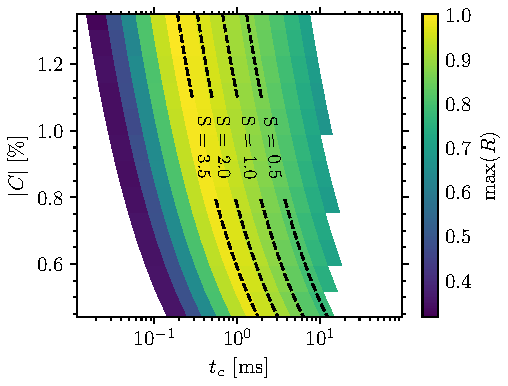
\includegraphics[width=0.85\linewidth]{THPOPT056_f1.pdf}
    \caption{Emittance exchange quality as function of coupling coefficient modulus $|C|$ and the time to cross the difference resonance $t_c$. The dashed lines indicate curves with constant $S$ and emittance exchange quality higher than $\SI{80}{\%}$}
    \label{fig:r_map}
\end{figure}
% The simulations were performed using Pyaccel~\cite{SaPyaccel}, a Python package for optics and tracking simulations developed by LNLS Accelerator Physics Group. 

Figure~\ref{fig:phase_space} shows the simulation results of the TEE effect, considering $R=\SI{95}{\%}$, on the injected beam after passing through the NLK under different injection positions. %\
% simulations results of comparing two bunches, one  with and other without TEE passing through the NLK, in different injection conditions.
The gray curves are the horizontal acceptance of the ring crossing $x'=0$ at $x = \SI{-8.5}{\milli \meter}$ at the NLK position, representing the measured dynamic aperture of the SR, and the dot-dashed lines are the required NLK pulse to deliver the bunch with $\expval{x'} \approx 0$.

One can observe that the exchange could avoid particle losses at injection, %\
either by increasing the distance between the injected beam and the aperture limits, in case of injection at $\SI{-8.5}{\milli \meter}$, or, by reducing the horizontal spread at the innermost injections ($x_0 > \SI{-8}{\milli \meter}$). %\
 
In all simulated injections, the correspondent increase of vertical beam size induced by TEE does not exceeds the vertical aperture limits.
\begin{figure}%[ht]
    \centering
    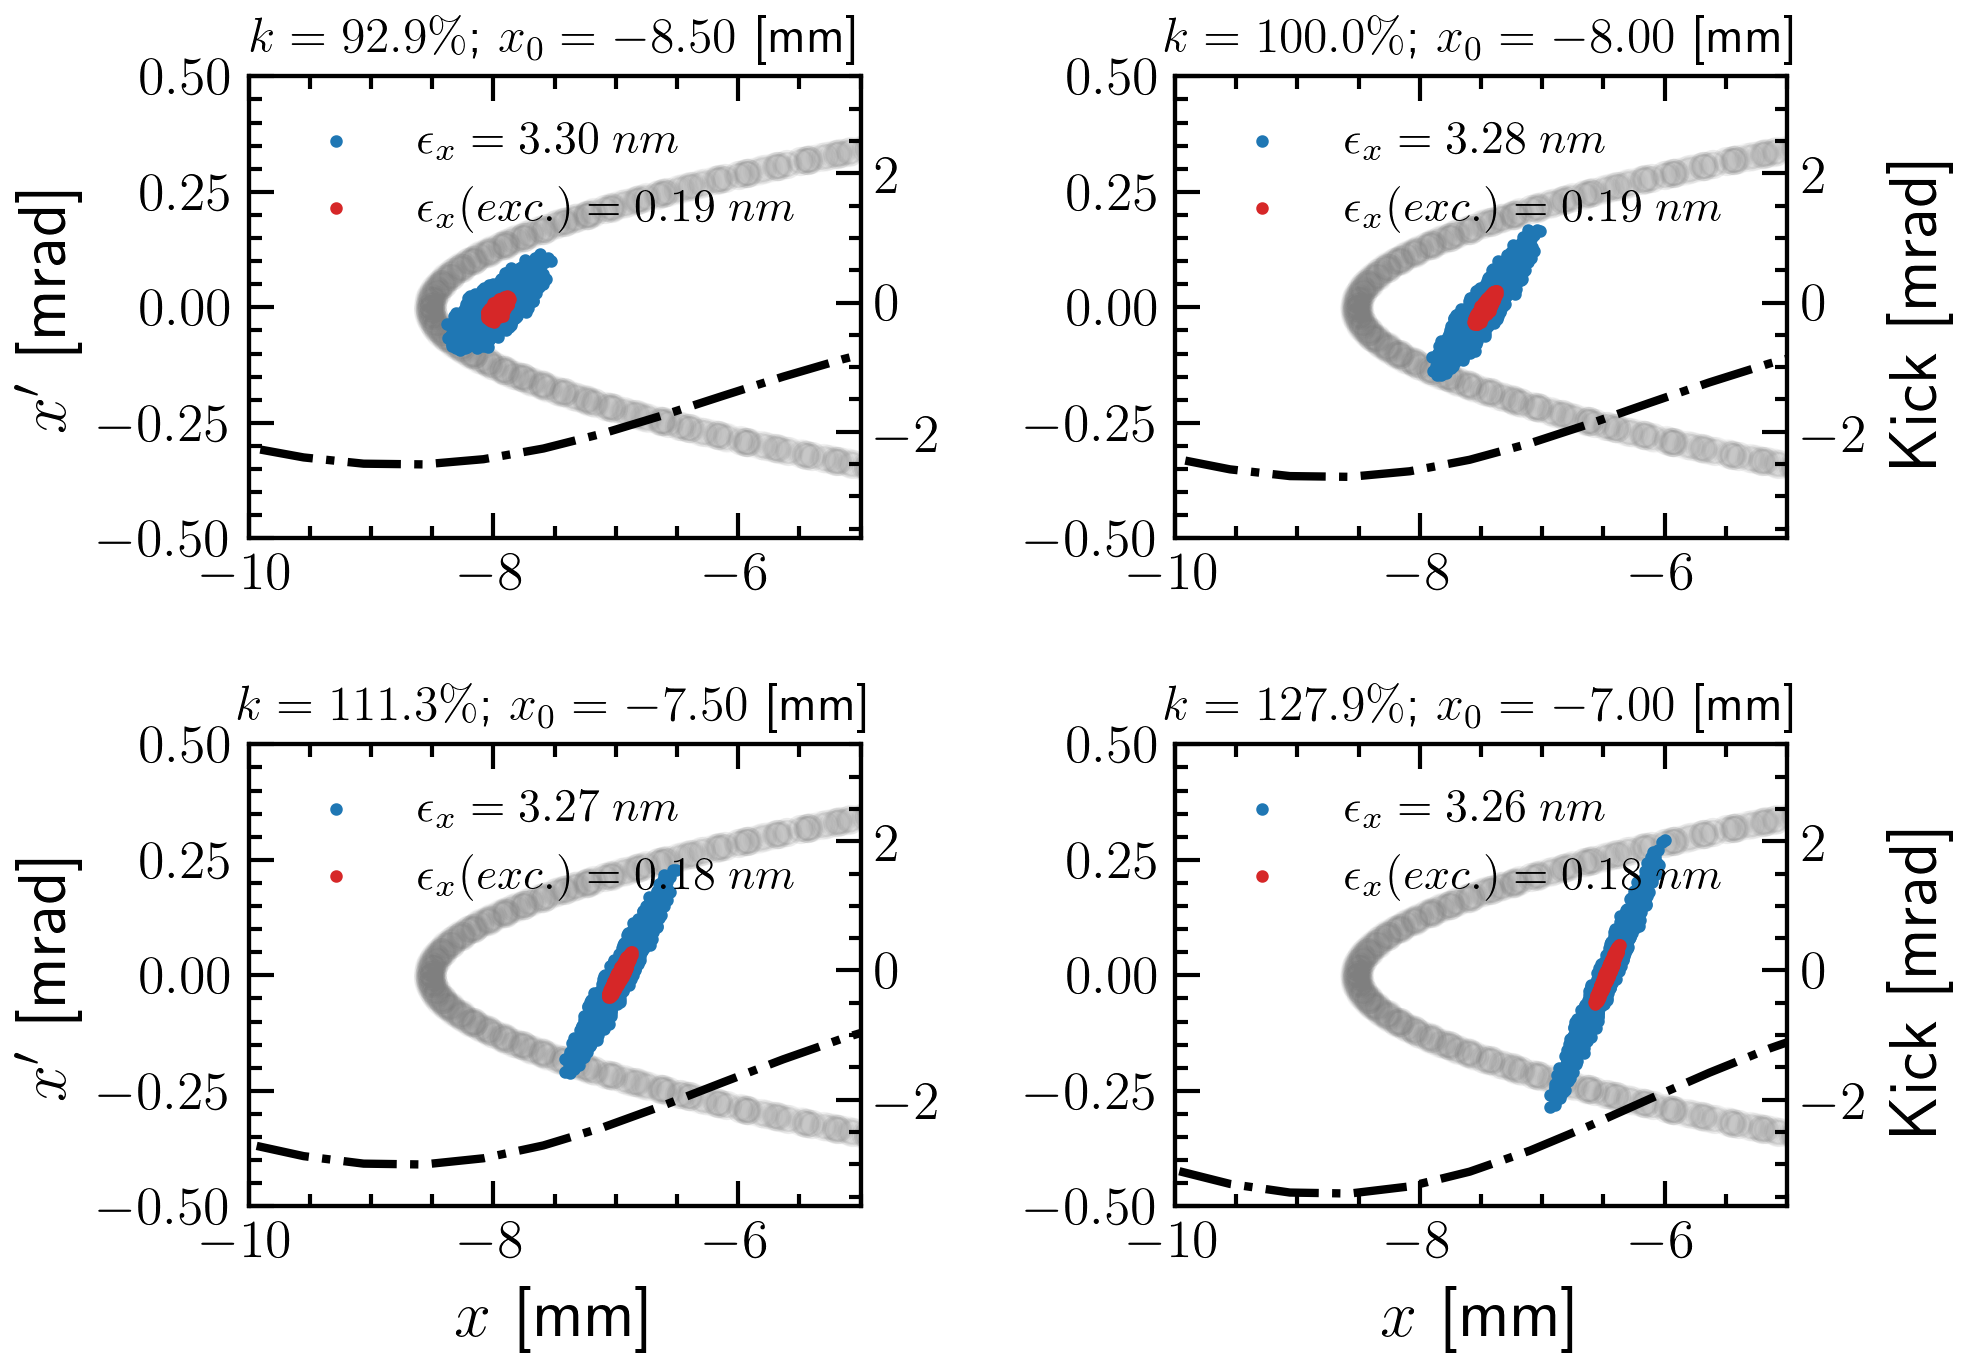
\includegraphics[width=\linewidth]{THPOPT056_f2.png}
    \caption{Phase-space diagrams of the bunch after the NLK for different initial horizontal positions $x_0$ at the NLK entrance. The dash-dotted lines represent the NLK pulse in units of angular kick. At each initial position, the NLK kick was optimized to deliver the bunch with $\expval{x'} \approx 0$. The parameter $k$ express the pulse intensity relative to the pulse used to align the bunch with $x_0 = - \SI{8.00}{\milli \meter}$.}
    \label{fig:phase_space}
\end{figure}
\section{EMITTANCE EXCHANGE IMPLEMENTATION}

The SIRIUS booster ramps the beam energy from $\SI{150}{\mega \electronvolt}$ to $\SI{3}{\giga\electronvolt}$, with nominal betatron tunes $\nu_x = 19.204$, $\nu_y = 7.314$, energy spread $\sigma_{\delta} = \SI{0.087}{\%}$, damping times $\tau_x=\SI{11.3}{\milli\second}$, $\tau_y = \SI{13.7}{\milli\second}$, natural emittance $\epsilon_0 = \SI{3.5}{\nano \meter\radian}$ at $\SI{3}{\giga\electronvolt}$, and ramp duration of approximately $\SI{300}{\milli\second}$, with repetition rate of $\SI{2}{\hertz}$.

Applying the closest tune approach method by using the family of defocusing quadrupoles (QD) in Booster to scan the tunes, we find a natural betatron coupling of $|C|=\SI{0.6 \pm 0.3}{\%}$, as showed in the Fig.~\ref{fig:coupling_exp}. The tunes were measured by first exciting betatron oscillations with the booster extraction kicker and then performing a frequency analysis of position data provided by the BPMs. %
% from the frequency analysis of position data provided by the BPMs after exciting betatron oscillations with the booster extraction kicker
With this measured coupling value we were able to analyze the TEE efficiency map of Fig.~\ref{fig:r_map} to conclude that reasonable values for $t_c$ should be within the interval $\SI{0.6}{\milli \second}<t_c<\SI{4}{\milli \second}$.
\begin{figure}%[ht]
    \centering
    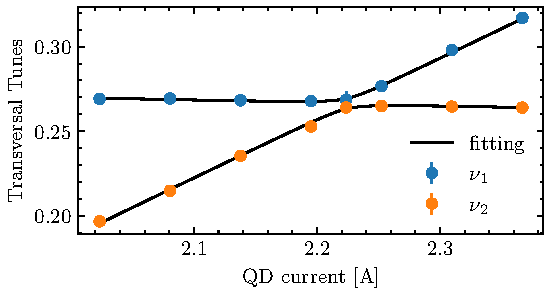
\includegraphics[width=0.85\linewidth]{THPOPT056_f3.pdf}
    \caption{Closest tune approach method for measurement of natural betatron coupling close to extraction energy.}
    \label{fig:coupling_exp}
\end{figure}

The TEE implementation was made by changing the QD-quadrupole current ramp to provide the tune crossing resonance approximately $\SI{1}{\milli \second}$ before beam extraction~\cite{Kallestrup2020}, as shown in Fig.~\ref{fig:bo_ramps}.
\begin{figure}[ht]
    \centering
    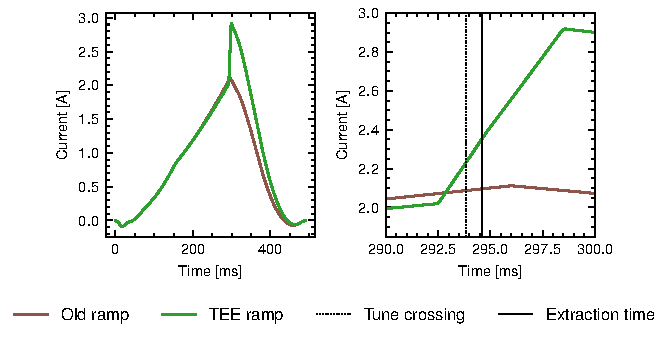
\includegraphics[width=0.9\linewidth]{THPOPT056_f4.pdf}
    \caption{Modification made in QD quadrupoles current ramp to implement the TEE. On the left, the full ramp is shown and a zoom with the details around the extraction point is on the right plot.}
    \label{fig:bo_ramps}
\end{figure}
%%
\subsection{Evaluating the exchange quality}
%%
The time $t_{ext}$ in which the derivative change occurs in the ramp was scanned from $\qtyrange{-3}{+3}{\milli \second}$ relative to the extraction time, %\
% Negative values above $\approx = \SI{-1}{\milli \second}$ for this time means that the beam was extracted from booster before any change in the quadrupole current derivative.
and the beam sizes were measured at the YAG screen in the booster-to-SR transport line. The results are displayed in Fig.~\ref{subfig:emit_exc_beamsizes} and show the TEE effect on the beam sizes. Notice that in the nominal extracting configuration, the horizontal beam size is reduced by a factor of $\approx 1.5$.

In Fig.~\ref{subfig:emit_exc_emittances} an estimate of the emittances during the TEE process is shown. This calculation was made with Eq. \eqref{eq:emit_by_beamsize},
\begin{equation}
    \epsilon_{x, y} = \frac{\sigma_{x, y}^2 - (\sigma_\delta \eta_{x,y})^2}{\beta_{x, y}},
    \label{eq:emit_by_beamsize}
\end{equation}
where the nominal values for energy spread $\sigma_\delta$, dispersion $\eta_{x,y}$ and betatron functions $\beta_{x, y}$ were used. The measured beam sizes $\sigma_{x, y}$ were used as inputs for Eq. \eqref{eq:emit_by_beamsize}. Based on this estimation, the TEE quality of the extracted beam is $R = \SI{70\pm10}{\%}$. With this estimate, it seems to be possible to improve the exchange quality with fine tuning of the parameters of TEE process in the booster ramp.

It is worth to mention that the emittances obtained from the previous estimation, both horizontally and vertically, are about 3 times higher in relation to our nominal model. The cause of this discrepancy is still unclear. Recent dispersion measurement values are close to expected from our nominal model, so they are not a probable source of this discrepancy. In addition, the YAG screen used is not designed for accurate beam size measurements and thus may yield larger sizes than the real ones.
\begin{figure}[ht]
\centering
\begin{subfigure}[c]{0.45\textwidth}
         \centering
         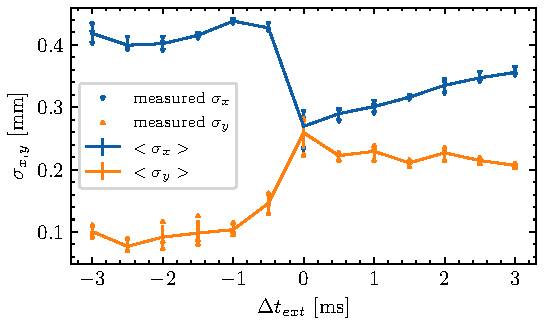
\includegraphics[trim={0.2cm 0.2cm 0 0}, clip, width=0.8\textwidth]{THPOPT056_f5a.pdf}
         \caption{Beam sizes during emittance exchange.}
         \label{subfig:emit_exc_beamsizes}
\end{subfigure}
\hfill
\begin{subfigure}[c]{0.45\textwidth}
        \centering
        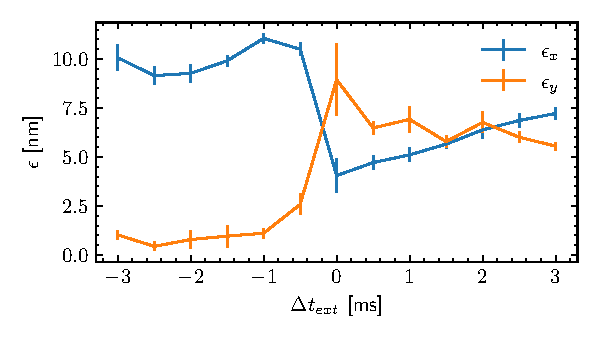
\includegraphics[trim={0.4cm 0.4cm 0 0}, clip, width=0.85\textwidth]{THPOPT056_f5b.pdf}
         \caption{Estimate of emittances behavior using nominal optical functions.}
         \label{subfig:emit_exc_emittances}
     \end{subfigure}
        \caption{Beam sizes and estimated emittances during the emittance exchange process. Measurements realized at YAG Screen in booster-to-SR transport line.  Design value for energy spread: $\sigma_{\delta} = \SI{0.087}{\%}$. Nominal optical functions used: $\beta_x = \SI{17.11}{\meter}$, $\beta_y = \SI{6.60}{\meter}$, $\eta_x = \SI{-13}{\centi \meter}$, $\eta_y = \SI{0}{\milli \meter}$.}
        \label{fig:vary_ext_times}
\end{figure}

\subsection{Injection efficiency}

With the optimized injection system for beam accumulation in the SIRIUS SR, which typically happens just after machine studies shifts, the median of injection efficiency was $\approx 86 \%$ before TEE implementation, being improved to about $96\%$ after TEE. However, we have been observing a degradation in the injection conditions during the injection for user shifts. Therefore, considering only the efficiency during injection for users, the median drops to $75 \%$ without TEE process, and to $82\%$ with the TEE settings in the ramp.

Furthermore, large pulse-to-pulse variations are being observed during beam accumulation at SR. This jitter causes an injection efficiency variation of about $10\%$. Besides, before the TEE implementation, the injection efficiency had a high correlation with the temperature drifts measured at the pulsed magnets used for injection. After the TEE, a lower correlation between injection efficiency and pulsed magnets temperatures was observed. This is probably related to the fact that with a smaller beam in horizontal, the injection is more robust against variations of injection conditions. This behavior is under study.

\section{CONCLUSION}

The use of TEE proved to be a valuable tool for the improvement of injection into SIRIUS SR, given the off-axis injection scheme difficulties due to limited dynamic aperture. In this paper, we discussed and presented the TEE implementation in the SIRIUS booster by crossing a tune difference resonance. Particle simulations showed that the TEE could prevent particle losses during off-axis injection with the NLK and beam envelope tracking indicated a set of appropriated parameters for the TEE in SIRIUS. The tune difference resonance crossing was performed by changing the defocusing quadrupoles strength at the end of the ramp.

Measurements realized in the YAG screen at booster to SR transport line have shown a horizontal beam size reduction by a factor of $\approx$ 1.5. The emittances were estimated using beam size measurements and nominal values for optical functions at transport line, the calculation suggests a exchange quality of about $\SI{70 \pm 10}{\%}$.

% An estimation of emittances was performed with the beam size measurements and nominal values for optics functions at transport line. The calculation suggests that the emittance exchange quality is about $\SI{70 \pm 10}{\%}$. The calculation suggests that the emittance exchange quality is about $\SI{70 \pm 10}{\%}$.

% Further experiments are planned, exploring different parameters for the TEE, for example, different crossing velocities to improve the exchange quality.

The TEE implementation increased the SR injection efficiency from 86\% to 96\% on average when the injection system is optimized. The relation between TEE implementation and injection efficiency robustness against jitters and drifts on the injection conditions is under investigation.

\section{ACKNOWLEDGEMENTS}
The authors thank to Liu Lin and Ximenes Resende for suggesting the work and valuable support.
%
% only for "biblatex"
%
% \newpage
\ifboolexpr{bool{jacowbiblatex}}%
	{\printbibliography}%
	{%
	% "biblatex" is not used, go the "manual" way
	
	\begin{thebibliography}{99}   % Use for  10-99  references
% 	\begin{thebibliography}{9} % Use for 1-9 references
	
  \bibitem{Liu:IPAC16-THPMR011}
  L. Liu, X. R. Resende, A. R. D. Rodrigues, and F. H. de Sá,
  \textquotedblleft{Injection Dynamics for Sirius Using a Nonlinear Kicker}\textquotedblright,
  in \emph{Proc. IPAC’16}, Busan, Korea, May 2016, pp. 3406--3408.
  \url{doi:10.18429/JACoW-IPAC2016-THPMR011}
	
    \bibitem{Liu:IPAC14-WEPRO009}
   L. Liu, X. R. Resende, A. R. D. Rodrigues, and F. H. de Sá,
   \textquotedblleft{A New Booster Synchrotron for the Sirius Project}\textquotedblright,
   in \emph{Proc. IPAC’14}, Dresden, Germany, Jun. 2014, pp. 1959--1961.
   \url{doi:10.18429/JACoW-IPAC2014-WEPRO009}            
	
    \bibitem{Dester:IPAC17-WEPIK052}
   P. S. Dester, L. Liu, and F. H. de Sá,
   \textquotedblleft{Energy Acceptance and on Momentum Aperture Optimization for the Sirius Project}\textquotedblright,
   in \emph{Proc. IPAC’17}, Copenhagen, Denmark, May 2017, pp. 3041--3044.
   \url{doi:10.18429/JACoW-IPAC2017-WEPIK052}
   
   \bibitem{Resende:IPAC22-THPOPT038}
 X. R. Resende, et al., \textquotedblleft{Sirius Injection Optimization}\textquotedblright,
  presented at the 13th International Particle Accelerator Conf. (IPAC’22), Bangkok, Thailand, Jun. 2022, paper THPOPT038, this conference.
   
    \bibitem{Kuske:IPAC16-WEOAA01}
  P. Kuske and F. Kramer,
  \textquotedblleft{Transverse Emittance Exchange for Improved Injection Efficiency}\textquotedblright,
  in \emph{Proc. IPAC’16}, Busan, Korea, May 2016, pp. 2028--2031.
  \url{doi:10.18429/JACoW-IPAC2016-WEOAA01}            
  %\cite{Kallestrup:IPAC21-MOPAB020}
  \bibitem{Kallestrup:IPAC21-MOPAB020}
  J. Kallestrup and M. Aiba,
  \textquotedblleft{Improvements to the SLS Booster Synchrotron Performance Towards SLS 2.0}\textquotedblright,
  in \emph{Proc. IPAC’21}, Campinas, Brazil, May 2021, pp. 103--106.
  \url{doi:10.18429/JACoW-IPAC2021-MOPAB020}     
  %\cite{Carmignani:IPAC21-MOPAB051}
    \bibitem{Carmignani:IPAC21-MOPAB051}
  N. Carmignani, L. R. Carver, S. M. Liuzzo, T. P. Perron, and S. M. White,
  \textquotedblleft{Operation of the ESRF Booster with the New EBS Storage Ring}\textquotedblright,
  in \emph{Proc. IPAC’21}, Campinas, Brazil, May 2021, pp. 221--224.
  \url{doi:10.18429/JACoW-IPAC2021-MOPAB051}  
	
  \bibitem{Kallestrup2020}
  J. Kallestrup and M. Aiba,
  \textquotedblleft{Emittance exchange in electron booster synchrotron by coupling resonance crossing}\textquotedblright,
  \emph{Phys. Rev. ST Accel. Beams}, vol. 23, no. 2, p. 020701, Feb. 2020, 
  \url{doi: 10.1103/PhysRevAccelBeams.23.020701}
    
    \bibitem{Aiba2020}
    M. Aiba and J. Kallestrup,
    \textquotedblleft{Theory of emittance exchange
    through coupling resonance crossing}\textquotedblright,
    \emph{Phys. Rev. ST Accel. Beams}, vol. 23, no. 4, p. 44003, 2020, 
    \url{10.1103/PhysRevAccelBeams.23.044003}
    
    \bibitem{Guignard1995}
    G. Guignard,
    \textquotedblleft{Betatron coupling and related impact of radiation}\textquotedblright,
    \emph{Phys. Rev. E}, vol. 51, no. 6, p. 6104, 1995, 
    \url{doi:10.1103/PhysRevE.51.6104}
    
    %\cite{Capoani:IPAC21-TUPAB232}
    \bibitem{Capoani:IPAC21-TUPAB232}
   F. Capoani, A. Bazzani, M. Giovannozzi, and A. I. Neishtadt,
   \textquotedblleft{Linear Coupling and Adiabaticity of Emittance Exchange}\textquotedblright,
   in \emph{Proc. IPAC’21}, Campinas, Brazil, May 2021, pp. 1972--1975.
   \url{doi:10.18429/JACoW-IPAC2021-TUPAB232}
   
   
    \bibitem{Ohmi1994}
    K. Ohmi, K. Hirata, and K. Oide, 
     \textquotedblleft{From the beam-envelope matrix to synchrotron-radiation integrals}\textquotedblright,
    \emph{Phys. Rev. E}, vol. 49, no. 1, pp. 751–765, 1994.
    \url{doi:10.1103/PhysRevE.49.751}
    
    
	\end{thebibliography}
} 
%
% for use as JACoW template the inclusion of the ANNEX parts have been commented out
% to generate the complete documentation please remove the "%" of the next two commands
% 

%\include{annexes-A4}

\end{document}
